\documentclass[]{book}
\usepackage{lmodern}
\usepackage{amssymb,amsmath}
\usepackage{ifxetex,ifluatex}
\usepackage{fixltx2e} % provides \textsubscript
\ifnum 0\ifxetex 1\fi\ifluatex 1\fi=0 % if pdftex
  \usepackage[T1]{fontenc}
  \usepackage[utf8]{inputenc}
\else % if luatex or xelatex
  \ifxetex
    \usepackage{mathspec}
  \else
    \usepackage{fontspec}
  \fi
  \defaultfontfeatures{Ligatures=TeX,Scale=MatchLowercase}
\fi
% use upquote if available, for straight quotes in verbatim environments
\IfFileExists{upquote.sty}{\usepackage{upquote}}{}
% use microtype if available
\IfFileExists{microtype.sty}{%
\usepackage{microtype}
\UseMicrotypeSet[protrusion]{basicmath} % disable protrusion for tt fonts
}{}
\usepackage{hyperref}
\hypersetup{unicode=true,
            pdftitle={Network Analysis in R},
            pdfborder={0 0 0},
            breaklinks=true}
\urlstyle{same}  % don't use monospace font for urls
\usepackage{natbib}
\bibliographystyle{apalike}
\usepackage{color}
\usepackage{fancyvrb}
\newcommand{\VerbBar}{|}
\newcommand{\VERB}{\Verb[commandchars=\\\{\}]}
\DefineVerbatimEnvironment{Highlighting}{Verbatim}{commandchars=\\\{\}}
% Add ',fontsize=\small' for more characters per line
\usepackage{framed}
\definecolor{shadecolor}{RGB}{248,248,248}
\newenvironment{Shaded}{\begin{snugshade}}{\end{snugshade}}
\newcommand{\AlertTok}[1]{\textcolor[rgb]{0.94,0.16,0.16}{#1}}
\newcommand{\AnnotationTok}[1]{\textcolor[rgb]{0.56,0.35,0.01}{\textbf{\textit{#1}}}}
\newcommand{\AttributeTok}[1]{\textcolor[rgb]{0.77,0.63,0.00}{#1}}
\newcommand{\BaseNTok}[1]{\textcolor[rgb]{0.00,0.00,0.81}{#1}}
\newcommand{\BuiltInTok}[1]{#1}
\newcommand{\CharTok}[1]{\textcolor[rgb]{0.31,0.60,0.02}{#1}}
\newcommand{\CommentTok}[1]{\textcolor[rgb]{0.56,0.35,0.01}{\textit{#1}}}
\newcommand{\CommentVarTok}[1]{\textcolor[rgb]{0.56,0.35,0.01}{\textbf{\textit{#1}}}}
\newcommand{\ConstantTok}[1]{\textcolor[rgb]{0.00,0.00,0.00}{#1}}
\newcommand{\ControlFlowTok}[1]{\textcolor[rgb]{0.13,0.29,0.53}{\textbf{#1}}}
\newcommand{\DataTypeTok}[1]{\textcolor[rgb]{0.13,0.29,0.53}{#1}}
\newcommand{\DecValTok}[1]{\textcolor[rgb]{0.00,0.00,0.81}{#1}}
\newcommand{\DocumentationTok}[1]{\textcolor[rgb]{0.56,0.35,0.01}{\textbf{\textit{#1}}}}
\newcommand{\ErrorTok}[1]{\textcolor[rgb]{0.64,0.00,0.00}{\textbf{#1}}}
\newcommand{\ExtensionTok}[1]{#1}
\newcommand{\FloatTok}[1]{\textcolor[rgb]{0.00,0.00,0.81}{#1}}
\newcommand{\FunctionTok}[1]{\textcolor[rgb]{0.00,0.00,0.00}{#1}}
\newcommand{\ImportTok}[1]{#1}
\newcommand{\InformationTok}[1]{\textcolor[rgb]{0.56,0.35,0.01}{\textbf{\textit{#1}}}}
\newcommand{\KeywordTok}[1]{\textcolor[rgb]{0.13,0.29,0.53}{\textbf{#1}}}
\newcommand{\NormalTok}[1]{#1}
\newcommand{\OperatorTok}[1]{\textcolor[rgb]{0.81,0.36,0.00}{\textbf{#1}}}
\newcommand{\OtherTok}[1]{\textcolor[rgb]{0.56,0.35,0.01}{#1}}
\newcommand{\PreprocessorTok}[1]{\textcolor[rgb]{0.56,0.35,0.01}{\textit{#1}}}
\newcommand{\RegionMarkerTok}[1]{#1}
\newcommand{\SpecialCharTok}[1]{\textcolor[rgb]{0.00,0.00,0.00}{#1}}
\newcommand{\SpecialStringTok}[1]{\textcolor[rgb]{0.31,0.60,0.02}{#1}}
\newcommand{\StringTok}[1]{\textcolor[rgb]{0.31,0.60,0.02}{#1}}
\newcommand{\VariableTok}[1]{\textcolor[rgb]{0.00,0.00,0.00}{#1}}
\newcommand{\VerbatimStringTok}[1]{\textcolor[rgb]{0.31,0.60,0.02}{#1}}
\newcommand{\WarningTok}[1]{\textcolor[rgb]{0.56,0.35,0.01}{\textbf{\textit{#1}}}}
\usepackage{longtable,booktabs}
\usepackage{graphicx,grffile}
\makeatletter
\def\maxwidth{\ifdim\Gin@nat@width>\linewidth\linewidth\else\Gin@nat@width\fi}
\def\maxheight{\ifdim\Gin@nat@height>\textheight\textheight\else\Gin@nat@height\fi}
\makeatother
% Scale images if necessary, so that they will not overflow the page
% margins by default, and it is still possible to overwrite the defaults
% using explicit options in \includegraphics[width, height, ...]{}
\setkeys{Gin}{width=\maxwidth,height=\maxheight,keepaspectratio}
\IfFileExists{parskip.sty}{%
\usepackage{parskip}
}{% else
\setlength{\parindent}{0pt}
\setlength{\parskip}{6pt plus 2pt minus 1pt}
}
\setlength{\emergencystretch}{3em}  % prevent overfull lines
\providecommand{\tightlist}{%
  \setlength{\itemsep}{0pt}\setlength{\parskip}{0pt}}
\setcounter{secnumdepth}{5}
% Redefines (sub)paragraphs to behave more like sections
\ifx\paragraph\undefined\else
\let\oldparagraph\paragraph
\renewcommand{\paragraph}[1]{\oldparagraph{#1}\mbox{}}
\fi
\ifx\subparagraph\undefined\else
\let\oldsubparagraph\subparagraph
\renewcommand{\subparagraph}[1]{\oldsubparagraph{#1}\mbox{}}
\fi

%%% Use protect on footnotes to avoid problems with footnotes in titles
\let\rmarkdownfootnote\footnote%
\def\footnote{\protect\rmarkdownfootnote}

%%% Change title format to be more compact
\usepackage{titling}

% Create subtitle command for use in maketitle
\providecommand{\subtitle}[1]{
  \posttitle{
    \begin{center}\large#1\end{center}
    }
}

\setlength{\droptitle}{-2em}

  \title{Network Analysis in R}
    \pretitle{\vspace{\droptitle}\centering\huge}
  \posttitle{\par}
    \author{}
    \preauthor{}\postauthor{}
      \predate{\centering\large\emph}
  \postdate{\par}
    \date{2019-12-07}

\usepackage{booktabs}

\newenvironment{danger}
    {
    \hline\\
    }
    { 
    \\\\\hline
    }
    
\newenvironment{warning}
    {
    \hline\\
    }
    { 
    \\\\\hline
    }
    
\newenvironment{info}
    {
    \hline\\
    }
    { 
    \\\\\hline
    }
    
\newenvironment{try}
    {
    \hline\\
    }
    { 
    \\\\\hline
    }
\usepackage{booktabs}
\usepackage{longtable}
\usepackage{array}
\usepackage{multirow}
\usepackage{wrapfig}
\usepackage{float}
\usepackage{colortbl}
\usepackage{pdflscape}
\usepackage{tabu}
\usepackage{threeparttable}
\usepackage{threeparttablex}
\usepackage[normalem]{ulem}
\usepackage{makecell}
\usepackage{xcolor}

\begin{document}
\maketitle

{
\setcounter{tocdepth}{1}
\tableofcontents
}
\hypertarget{overview}{%
\chapter*{Overview}\label{overview}}
\addcontentsline{toc}{chapter}{Overview}

Materials for the 4 day Network Analysis course.

This course covers skills such as installing R, opening fies, working with data using tidyverse, and making graphs. It also introduces network analysis as a statistical concept.

\hypertarget{starting-with-r}{%
\chapter{Starting with R}\label{starting-with-r}}

{Welcome to the Course!}

\hypertarget{overview-1}{%
\section{Overview}\label{overview-1}}

Installing R and opening files

\textbf{In this session you will learn:}

\begin{enumerate}
\def\labelenumi{\arabic{enumi}.}
\tightlist
\item
  What is R?
\item
  How to install R
\item
  Where to get help
\end{enumerate}

\hypertarget{what-is-r}{%
\subsection{What is R?}\label{what-is-r}}

For network analysis, you need two different bits of software, R and RStudio. R is a programming language that you will write code in and R Studio is an Integrated Development Environment (IDE) which makes working with R easier.

\hypertarget{how-to-install-base-r}{%
\subsection{How To Install Base R}\label{how-to-install-base-r}}

Install base R from \url{https://cran.rstudio.com/}. Choose the download link for your operating system (Linux, Mac OS X, or Windows).

\hypertarget{how-to-install-r-studio}{%
\subsection{How To Install R Studio}\label{how-to-install-r-studio}}

Go to \url{https://rstudio.com} and download the RStudio Desktop (Open Source License) version for your operating system under the list titled \textbf{Installers for Supported Platforms.}

If you are using a Mac, please install \href{https://www.xquartz.org/}{XQuartz}

\hypertarget{quiz}{%
\subsection{Quiz}\label{quiz}}

{Quickfire Questions}

We have put questions throughout to help you test your knowledge. When you type in or choose the correct answer, the dashed box will change color and become solid green.

\begin{itemize}
\tightlist
\item
  From the following options, how do you get R for this course? Installing Base R \& R Studio Installing R Studio Installing Base R
\end{itemize}

Explain This Answer!

R is the basic package. R Studio is an add-on that make R much easier to use.

\hypertarget{where-to-get-help}{%
\section{Where to Get Help}\label{where-to-get-help}}

Learning R can take time. Please do not feel that you have to grasp everything right away and it is totally ok to copy and paste.

\hypertarget{google}{%
\subsection{Google}\label{google}}

\textbf{``Never commit to memory what can be easily looked up in books''}

Often people simply google what they want to achieve in R. For example, in preparing this tutorial I googled ``how to run a linear mixed effects model in R'' (as I did not know) and found the following \href{https://ourcodingclub.github.io/2017/03/15/mixed-models.html}{helpful tutorial} which goes through all the steps. This is just one of many examples of resources that are available.

\hypertarget{stackoverflow}{%
\subsection{Stackoverflow}\label{stackoverflow}}

\href{https://stackoverflow.com}{Stackoverflow} is a website where you can ask for help on bits of coding that you are struggling with. You can search for commonly asked questions and responses.

Feel free to google any time.

\hypertarget{working-with-data-in-r}{%
\chapter{Working With Data in R}\label{working-with-data-in-r}}

\hypertarget{overview-2}{%
\section{Overview}\label{overview-2}}

{Working With Data}

\textbf{In this session you will learn:}

\begin{enumerate}
\def\labelenumi{\arabic{enumi}.}
\tightlist
\item
  How to open files
\item
  How to write code
\item
  How to install packages
\end{enumerate}

This is a basic introduction to R. The material is based on the data skills course for MSc students at the University of Glasgow. Find lots of useful resources here: \url{https://gupsych.github.io/data_skills/01_intro.html}

Please take a look at these free open resources in your own time.

\hypertarget{setting-working-directory}{%
\subsection{Setting Working Directory}\label{setting-working-directory}}

First things first, we will set the working directory. What this means is that we need to tell R where the files we need are located. Think of it just like when you have different projects, and you have seperate folders for each project e.g.~research conducted in schools, research conducted in the community and so on. When working on R, it's useful to have all the data sets and files you need in one folder.

To set the working directory press session -\textgreater{} set working directory -\textgreater{} choose directory and then select the folder where the data sets we are working on are saved, and save this file in the same folder as well. In other words- make sure your data sets and scripts are all in the same folder.

\hypertarget{code}{%
\subsection{Code}\label{code}}

RStudio generally has four panels: Current file, Console, Environment, and Viewer. You can think of the console as a place to try things out, and the file to write down ideas you want to stick around. Go to the console and type

\begin{Shaded}
\begin{Highlighting}[]
\NormalTok{x <-}\StringTok{ }\DecValTok{1} \OperatorTok{+}\StringTok{ }\DecValTok{5}
\NormalTok{x}
\end{Highlighting}
\end{Shaded}

Notice how now the environment shows we have a Value x that is 6. We have just created a variable. In the above, we would say ``the variable x is assigned to 1 + 5'' or ``x gets 1 + 5''

\hypertarget{functions-arguments}{%
\subsection{Functions \& Arguments}\label{functions-arguments}}

We have already created some code. But what does it all mean?

Functions in R execute specific tasks and normally take a number of arguments (if you're into linguistics you might want to think as these as verbs that require a subject and an object). You can look up all the arguments that a function takes by using the help documentation by using the format \texttt{?function}. Some arguments are required, and some are optional. Optional arguments will often use a default (normally specified in the help documentation) if you do not enter any value.

As an example, let's look at the help documentation for the function rnorm() which randomly generates a set of numbers with a normal distribution. Just like the numbers in the graph below.

Open up R Studio and in the console, type the following code:

\begin{Shaded}
\begin{Highlighting}[]
\NormalTok{?rnorm}
\end{Highlighting}
\end{Shaded}

The help documentation for \texttt{rnorm()} should appear in the bottom right help panel. In the usage section, we see that \texttt{rnorm()} takes the following form:

\begin{verbatim}
rnorm(n, mean = 0, sd = 1)
\end{verbatim}

In the arguments section, there are explanations for each of the arguments. \texttt{n} is the number of observations we want to create, \texttt{mean} is the mean of the data points we will create and \texttt{sd} is the standard deviation of the set. In the details section it notes that if no values are entered for mean and sd it will use a default of 0 and 1 for these values. Because there is no default value for n it must be specified otherwise the code won't run.

Now, try running the above code for 50 participants with a mean test score of 3 and a standard deviation of 1.

Remember we are asking R to create \textbf{random} numbers here, so do not worry if someone else has slightly different values.

I need a hint!

\texttt{n} in this case would be changed to 50.

\texttt{mean} should be changed to 3

\texttt{rnorm(50,\ mean\ =\ 3,\ sd\ =\ 1)}

now, try running the above code and see what happens.

\hypertarget{tidyverse}{%
\subsection{Tidyverse}\label{tidyverse}}

However, we do not always want to use R to create random numbers, we want to use it to analyse our own data which commonly resides in .csv or .sav files. People have developed many different libraries to help us work with such data. One of the most popular packages is tidyverse.

The Tidyverse is a collection of R packages with a common design , grammar, and data structure that makes analysis faster and easier.

The first time you want to use a package, you must first install the package. \texttt{tidyverse} can be installed as follows.

\begin{verbatim}
install.packages("tidyverse")
\end{verbatim}

Once the package has been installed, any time you want to use the package you use the following code. If you want to open a package other than \texttt{tidyverse}, simply substitute the package name.

\hypertarget{scripts}{%
\section{Scripts}\label{scripts}}

So far we have been typing into the console but that means all work is lost when re-start R. We can save our analysis code in scripts. To create a new script select the option from the File menu.

\hypertarget{opening-spss-files}{%
\subsection{Opening SPSS Files}\label{opening-spss-files}}

The \texttt{foreign} package allows easy opening of .sav files which are associated with SPSS.

You can either set a path to open up an SPSS file or run \texttt{file.choose()} and pick the file manually.

To use foreign, we need to first install the package, same as we did with tidyverse. Follow the instructions for installing tidyverse and subsitute the package name.

Click to see solution\ldots{}

\begin{verbatim}
install.packages("foreign")
\end{verbatim}

Once you have installed packages, .sav files can be opened using the following code:

\texttt{dataset\ =\ read.spss("YOURFILENAMEHERE.sav",\ to.data.frame=TRUE)}

While we are not using spss files during this training, it is useful to know how to do this.

\hypertarget{keeping-environment-clean}{%
\subsection{Keeping Environment Clean}\label{keeping-environment-clean}}

As you work, you will notice your environment will fill up with lots of variables that you have assigned.

Before beginning any new analyses it is important to clear the environment which can be done with the following code. If you run this code R will forget any libraries that you have loaded, such as \texttt{tidyverse}.

\begin{Shaded}
\begin{Highlighting}[]
\KeywordTok{rm}\NormalTok{(}\DataTypeTok{list =} \KeywordTok{ls}\NormalTok{())}
\end{Highlighting}
\end{Shaded}

\hypertarget{network-analysis}{%
\chapter{Network Analysis}\label{network-analysis}}

\hypertarget{overview-3}{%
\section{Overview}\label{overview-3}}

This session will cover the basics of network analysis approach. Check the references section for more advanced topics.

\hypertarget{background}{%
\section{Background}\label{background}}

Recent thinking conceptulises mental wellbeing as comprising of environmental, psychological and social factors, a challenge to static factor models. Psychologists wishing to study the dynamic interaction of many factors may wish to consider a complexity science perspective such as network analysis.

The potential utility of network analysis was noted over ten years ago in intelligence research. The frequently reported patterns of positive correlations between various cognitive tasks (e.g.~verbal comprehension and working memory) are typically explained in terms of a dominant latent factor, i.e.~the correlations reflect a hypothesised common factor of general intelligence (g). However, van der Maas (2006) and colleagues argued that this empirical pattern can also be accounted for by means of a network approach (see image below), wherein the patterns of positive relationships can be explained using a mutualism model, i.e.~the variables have mutual, reinforcing, relationships (Hevey, 2018)

The image above from van der Maas (2006) demonstrates the difference between a latent factor and a network approach.

\hypertarget{why-use-network-analysis-in-mental-health}{%
\section{Why Use Network Analysis in Mental Health?}\label{why-use-network-analysis-in-mental-health}}

``Analysis of mental health data is usually based on sum-scores of symptoms or the estimation of factor models. Both types of analyses disregard direct associations among symptoms that are well-understood in clinical practice: mental health problems can be conceptualized as vicious circles of problems that are hard to escape. A novel research framework, the network perspective on psychopathology, understands mental disorders as complex networks of interacting symptoms'' (Fried, 2018)

However, mental health networks can contain more than just symptoms. \href{https://jamanetwork.com/journals/jamapsychiatry/fullarticle/2671414?casa_token=nGUSw-yIg1YAAAAA\%3aXJz4Ehq44lBBE3iDqQhuNSGgJfafMX9lGyiDx9YxHJpVSFVOJo0gkA0NdrEGhY9T-6mvlB17}{In a study looking at patients with schizophrenia} the researchers wanted to understand the extent to which variables belonging to the same construct were connected and how different constructs mutually interacted and reinforced one another. In addition to modelling symptoms, the researchers also looked at engagement with mental health services and interpersonal relationships. This is important when we want to explore what wider influences might impact upon behaviour we are interested in.

\hypertarget{what-is-a-network}{%
\section{What is a network?}\label{what-is-a-network}}

A network is a set of nodes connected by a set of edges. A network (as collection of various nodes and edges) is also sometimes known as a graph.

A node (in psychological research) can represent a single item from a scale, a sub-scale, or a composite scale: the choice of node depends upon the type of data that provide the most appropriate and useful understanding of the questions to be addressed. Edges can represent different types of relationships, e.g.~co-morbidity of psychological symptoms.

Several packages are used in the network analysis, including \texttt{network}, \texttt{statnet}, \texttt{igraph} and \texttt{qgraph}.

qgraph was developed in the context of psychometrics approach by Dr.~Sacha Epskamp and colleagues in 2012. We will be be working with \texttt{qgraph} and \texttt{bootnet}. Please \texttt{install.packages("qgraph")} (which we will use now) and `install.packages(``bootnet'') (which we will use later) so we can get started.

Now, let us load up \texttt{qgraph} - remember and save all of your code into a script.

\begin{Shaded}
\begin{Highlighting}[]
\KeywordTok{library}\NormalTok{(qgraph)}
\end{Highlighting}
\end{Shaded}

\hypertarget{drawing-matrices}{%
\section{Drawing Matrices}\label{drawing-matrices}}

First, we will create a blank matrix with the following code. Here, we are asking R to create a matrix with 3 rows and 3 columns.

The code \texttt{colnames(Matrix)\ \textless{}-\ c("Node1","Node2","Node3")} is simply providing column names in the order they are created.

We can see that we have created a 3x3 matrix with no data.

\begin{Shaded}
\begin{Highlighting}[]
\NormalTok{Matrix <-}\StringTok{ }\KeywordTok{matrix}\NormalTok{(}\DecValTok{0}\NormalTok{,}\DataTypeTok{nrow=}\DecValTok{3}\NormalTok{,}\DataTypeTok{ncol=}\DecValTok{3}\NormalTok{)}
\KeywordTok{colnames}\NormalTok{(Matrix) <-}\StringTok{ }\KeywordTok{c}\NormalTok{(}\StringTok{"Node1"}\NormalTok{,}\StringTok{"Node2"}\NormalTok{,}\StringTok{"Node3"}\NormalTok{)}
\NormalTok{Matrix}
\end{Highlighting}
\end{Shaded}

\begin{verbatim}
##      Node1 Node2 Node3
## [1,]     0     0     0
## [2,]     0     0     0
## [3,]     0     0     0
\end{verbatim}

Now, we would like to assign some data to the matrix. We are mapping edges between nodes. For example, in the first line of code below ``3'' is the weighted edge between node 1 and 2.

\begin{Shaded}
\begin{Highlighting}[]
\NormalTok{Matrix[}\DecValTok{1}\NormalTok{,}\DecValTok{2}\NormalTok{] <-}\StringTok{ }\DecValTok{3}
\NormalTok{Matrix[}\DecValTok{2}\NormalTok{,}\DecValTok{1}\NormalTok{] <-}\StringTok{ }\DecValTok{3}
\NormalTok{Matrix[}\DecValTok{2}\NormalTok{,}\DecValTok{3}\NormalTok{] <-}\StringTok{ }\DecValTok{3}
\NormalTok{Matrix[}\DecValTok{3}\NormalTok{,}\DecValTok{2}\NormalTok{] <-}\StringTok{ }\DecValTok{3}
\NormalTok{Matrix}
\end{Highlighting}
\end{Shaded}

\begin{verbatim}
##      Node1 Node2 Node3
## [1,]     0     3     0
## [2,]     3     0     3
## [3,]     0     3     0
\end{verbatim}

\begin{Shaded}
\begin{Highlighting}[]
\KeywordTok{qgraph}\NormalTok{(Matrix)}
\end{Highlighting}
\end{Shaded}

\begin{figure}

{\centering 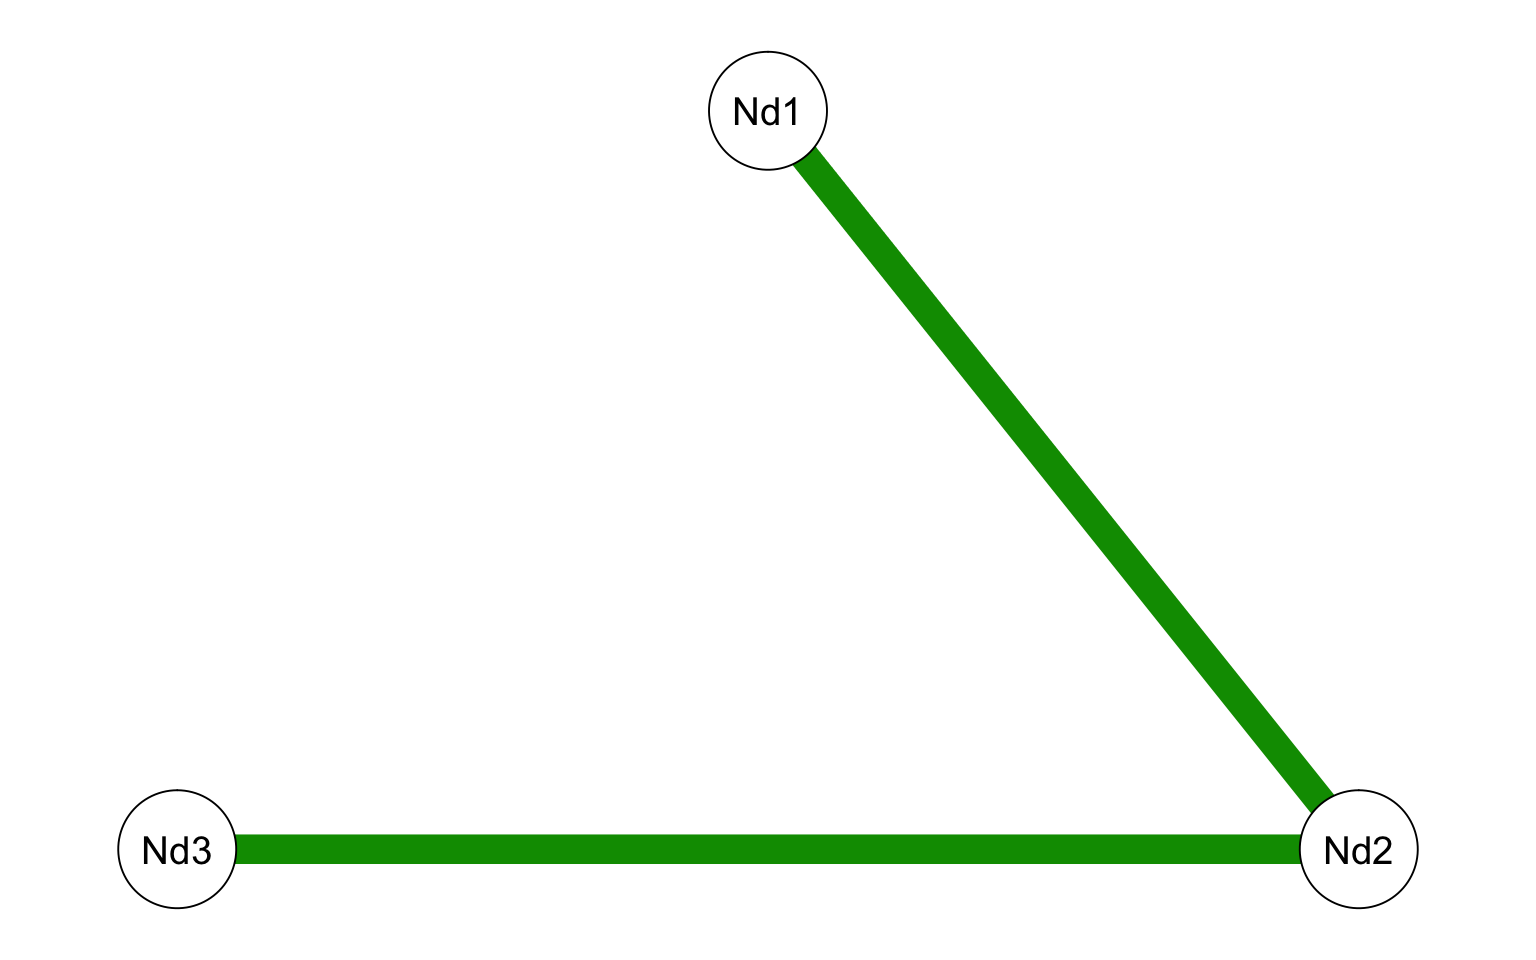
\includegraphics[width=1\linewidth]{03-s01-lab02a_files/figure-latex/qgraph-1} 

}

\caption{Matrix Visualisation}\label{fig:qgraph}
\end{figure}

\hypertarget{task}{%
\section{Task}\label{task}}

Change the Matrix values and visualise the result using qgraph. Feel free to try negative numbers too.

Click to see one possible example\ldots{}

\begin{Shaded}
\begin{Highlighting}[]
\NormalTok{Matrix[}\DecValTok{1}\NormalTok{,}\DecValTok{2}\NormalTok{] <-}\StringTok{ }\DecValTok{3}
\NormalTok{Matrix[}\DecValTok{2}\NormalTok{,}\DecValTok{1}\NormalTok{] <-}\StringTok{ }\DecValTok{3}
\NormalTok{Matrix[}\DecValTok{2}\NormalTok{,}\DecValTok{3}\NormalTok{] <-}\StringTok{ }\DecValTok{-3}
\NormalTok{Matrix[}\DecValTok{3}\NormalTok{,}\DecValTok{2}\NormalTok{] <-}\StringTok{ }\DecValTok{3}

\KeywordTok{qgraph}\NormalTok{(Matrix)}
\end{Highlighting}
\end{Shaded}

\begin{figure}

{\centering 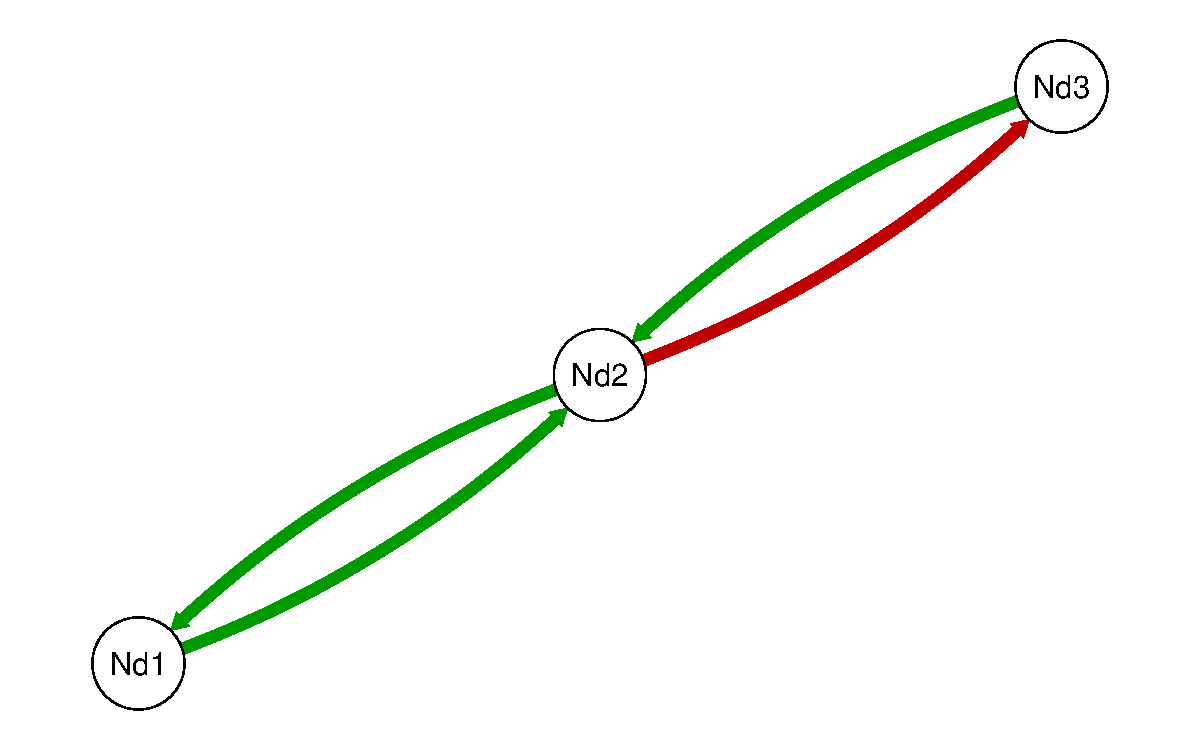
\includegraphics[width=1\linewidth]{03-s01-lab02a_files/figure-latex/unnamed-chunk-2-1} 

}

\caption{One Example - Change Numbers to see what happens}\label{fig:unnamed-chunk-2}
\end{figure}

\hypertarget{practical}{%
\chapter{Practical}\label{practical}}

\textbf{In this session you will learn:}

\begin{enumerate}
\def\labelenumi{\arabic{enumi}.}
\tightlist
\item
  How to work with original data
\item
  How to define factors
\item
  How to wrangle data
\item
  How to visualise data
\item
  How to run a simple network analysis.
\end{enumerate}

\hypertarget{description-of-data}{%
\section{Description of Data}\label{description-of-data}}

We will work with a local dataset gathered from high school age children. Please download the .csv file \href{data/networkdataset.csv}{HERE} (you might need to right click and choose save as).

First, we need to make sure we have \texttt{tidyverse} loaded and then open the file. We are creating a data frame called which we will assign to our .csv file.

Remember, this needs to be saved within the working directory that you set so that R knows where to find it.

\begin{Shaded}
\begin{Highlighting}[]
\KeywordTok{library}\NormalTok{(tidyverse)}
\KeywordTok{library}\NormalTok{(bootnet)}
\KeywordTok{library}\NormalTok{(qgraph)}
\KeywordTok{library}\NormalTok{(summarytools)}
\NormalTok{data <-}\StringTok{ }\KeywordTok{read_csv}\NormalTok{(}\StringTok{"networkdataset.csv"}\NormalTok{)}
\end{Highlighting}
\end{Shaded}

R has the \texttt{str()} function which lets us look at the structure of data. Look at \texttt{str(data)}

As we can see, Gender, Place and Grade are listed as character data (words), this is not accurate and it would be better to let R know these data are factors.

\begin{Shaded}
\begin{Highlighting}[]
\NormalTok{data_factors <-}\StringTok{ }\NormalTok{data }\OperatorTok
\StringTok{  }\KeywordTok{mutate}\NormalTok{(}\DataTypeTok{Gender =} \KeywordTok{as.factor}\NormalTok{(Gender),}
         \DataTypeTok{Place =} \KeywordTok{as.factor}\NormalTok{(Place),}
         \DataTypeTok{Grade =} \KeywordTok{as.factor}\NormalTok{(Grade),}
         \DataTypeTok{Familyarrangement =} \KeywordTok{as.factor}\NormalTok{(Familyarrangement),}
         \DataTypeTok{Average =} \KeywordTok{as.factor}\NormalTok{(Average),}
         \DataTypeTok{educationFather =} \KeywordTok{as.factor}\NormalTok{(educationFather),}
         \DataTypeTok{educationMather =} \KeywordTok{as.factor}\NormalTok{(educationMather))}
\end{Highlighting}
\end{Shaded}

Now, if we run \texttt{str(data\_factors)} we can see that this dataframe is recognised as factors.

\hypertarget{visualising-data}{%
\section{Visualising Data}\label{visualising-data}}

To do - write a bit about plotting options in R.

\hypertarget{visualising-data---practical}{%
\section{Visualising Data - Practical}\label{visualising-data---practical}}

How many females and males?

The \# symbol in the code is a comment. Comments do not add anything to the code but are there for human understanding to explain what is happening in the code. Look at the comments in the code below to understand what is going on.

\begin{Shaded}
\begin{Highlighting}[]
\CommentTok{# we are telling R we want to plot dat, we are letting R know Gender }
\CommentTok{# is a factor on our x axis and we want to fill with colour}
\KeywordTok{ggplot}\NormalTok{(data_factors, }\KeywordTok{aes}\NormalTok{(}\DataTypeTok{x =}\NormalTok{ Gender, }\DataTypeTok{fill =}\NormalTok{ Gender)) }\OperatorTok{+}
\StringTok{  }\CommentTok{# we are choosing a bar plot}
\StringTok{  }\KeywordTok{geom_bar}\NormalTok{(}\DataTypeTok{show.legend =} \OtherTok{FALSE}\NormalTok{, }\DataTypeTok{alpha =} \FloatTok{.8}\NormalTok{) }\OperatorTok{+}
\StringTok{  }\CommentTok{# we are naming the x scale}
\StringTok{  }\KeywordTok{scale_x_discrete}\NormalTok{(}\DataTypeTok{name =} \StringTok{"Gender"}\NormalTok{) }\OperatorTok{+}
\StringTok{  }\CommentTok{# we are chosing a colour scheme from pre-exising options}
\StringTok{  }\KeywordTok{scale_fill_viridis_d}\NormalTok{(}\DataTypeTok{option =} \StringTok{"D"}\NormalTok{) }\OperatorTok{+}
\StringTok{  }\CommentTok{# we are naming the y scale}
\StringTok{  }\KeywordTok{scale_y_continuous}\NormalTok{(}\DataTypeTok{name =} \StringTok{"Number of participants"}\NormalTok{)}
\end{Highlighting}
\end{Shaded}

\begin{figure}

{\centering 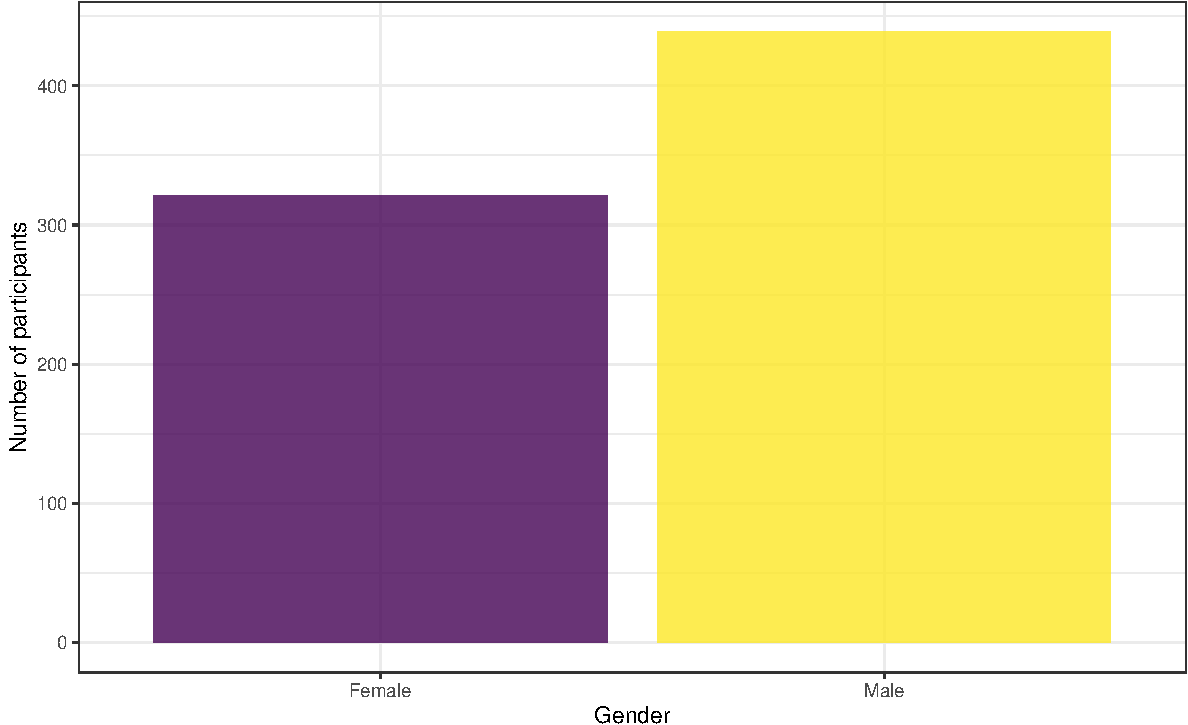
\includegraphics[width=1\linewidth]{04-s01-lab02a_files/figure-latex/graph-1} 

}

\caption{Participant Gender}\label{fig:graph}
\end{figure}

\hypertarget{working-with-data}{%
\section{Working With Data}\label{working-with-data}}

Participants rated themselves on 23 items of the TEQ questionnaire which asked about exposure to different traumatic events. We would like to create a plot to visualise the total TEQ and where participants live. However, we need to clean the data a little bit first. We will explain each line in the code below.

The pipe operator \%\textgreater{}\% is something you will see a lot and (in terms of code) means ``and then''

\begin{enumerate}
\def\labelenumi{\arabic{enumi}.}
\tightlist
\item
  we create a new dataframe called \texttt{total\_TEQ} which we assign to our new code
\item
  we then use \texttt{select}, the . lets R know we are still working with the same dataframe. We then select all TEQ variables, Pcode and Place \texttt{select(.,\ TEQ1:TEQ23,\ Pcode,\ Place}
\item
  \texttt{gather} tranforms the data from wide to long. We only want it to do this to TEQ variables so we can drop \texttt{-Pcode} and \texttt{-Place} using the minus sign.
\item
  We then use \texttt{group\_by(Pcode,\ Place)} as we want to look at scores for each participant and where they live
\item
  Finally \texttt{summarise(tot\_TEQ\ =\ sum(score))} creates a column named tot\_TEQ which has the total TEQ score for each participant.
\end{enumerate}

\begin{Shaded}
\begin{Highlighting}[]
\NormalTok{total_TEQ <-}\StringTok{ }\NormalTok{data_factors }\OperatorTok
\KeywordTok{select}\NormalTok{(., TEQ1}\OperatorTok{:}\NormalTok{TEQ23, Pcode, Place) }\OperatorTok
\KeywordTok{gather}\NormalTok{(}\StringTok{"var"}\NormalTok{, }\StringTok{"score"}\NormalTok{, }\OperatorTok{-}\NormalTok{Pcode, }\OperatorTok{-}\NormalTok{Place) }\OperatorTok
\KeywordTok{group_by}\NormalTok{(Pcode, Place) }\OperatorTok
\KeywordTok{summarise}\NormalTok{(}\DataTypeTok{tot_TEQ =} \KeywordTok{sum}\NormalTok{(score))}
\end{Highlighting}
\end{Shaded}

\hypertarget{plotting-data}{%
\section{Plotting Data}\label{plotting-data}}

Now we can visualise \texttt{total\_TEQ}.

When visualising differences between groups in numerical values, people have historically used bar graphs. There is currently a shift taking place, with people moving away from bar graphs, and towards more informative visualisations.

Before we used \texttt{geom\_bar()} to create a barplot and this time we will use \texttt{geom\_violin()} to create a violin plot. In the violin plot, the width of the area indicates the density of the data at that point on the y axis. We have also included a box plot using \texttt{geom\_boxplot} within this graph to show another option.

\begin{Shaded}
\begin{Highlighting}[]
\KeywordTok{ggplot}\NormalTok{(total_TEQ, }\KeywordTok{aes}\NormalTok{(}\DataTypeTok{x =} \KeywordTok{as.factor}\NormalTok{(Place), }\DataTypeTok{fill =} \KeywordTok{as.factor}\NormalTok{(Place), }\DataTypeTok{y =}\NormalTok{ tot_TEQ)) }\OperatorTok{+}\StringTok{ }\KeywordTok{geom_violin}\NormalTok{(}\DataTypeTok{show.legend =} \OtherTok{FALSE}\NormalTok{, }\DataTypeTok{trim =} \OtherTok{TRUE}\NormalTok{, }\DataTypeTok{alpha =} \FloatTok{0.8}\NormalTok{) }\OperatorTok{+}
\StringTok{  }\KeywordTok{geom_boxplot}\NormalTok{(}\DataTypeTok{width =} \FloatTok{0.2}\NormalTok{, }\DataTypeTok{show.legend =} \OtherTok{FALSE}\NormalTok{) }\OperatorTok{+}
\StringTok{  }\KeywordTok{scale_y_continuous}\NormalTok{(}\DataTypeTok{name =} \StringTok{"Total TEQ"}\NormalTok{) }\OperatorTok{+}
\StringTok{  }\KeywordTok{scale_x_discrete}\NormalTok{(}\DataTypeTok{name =} \StringTok{"Place"}\NormalTok{)}
\end{Highlighting}
\end{Shaded}

\begin{figure}

{\centering 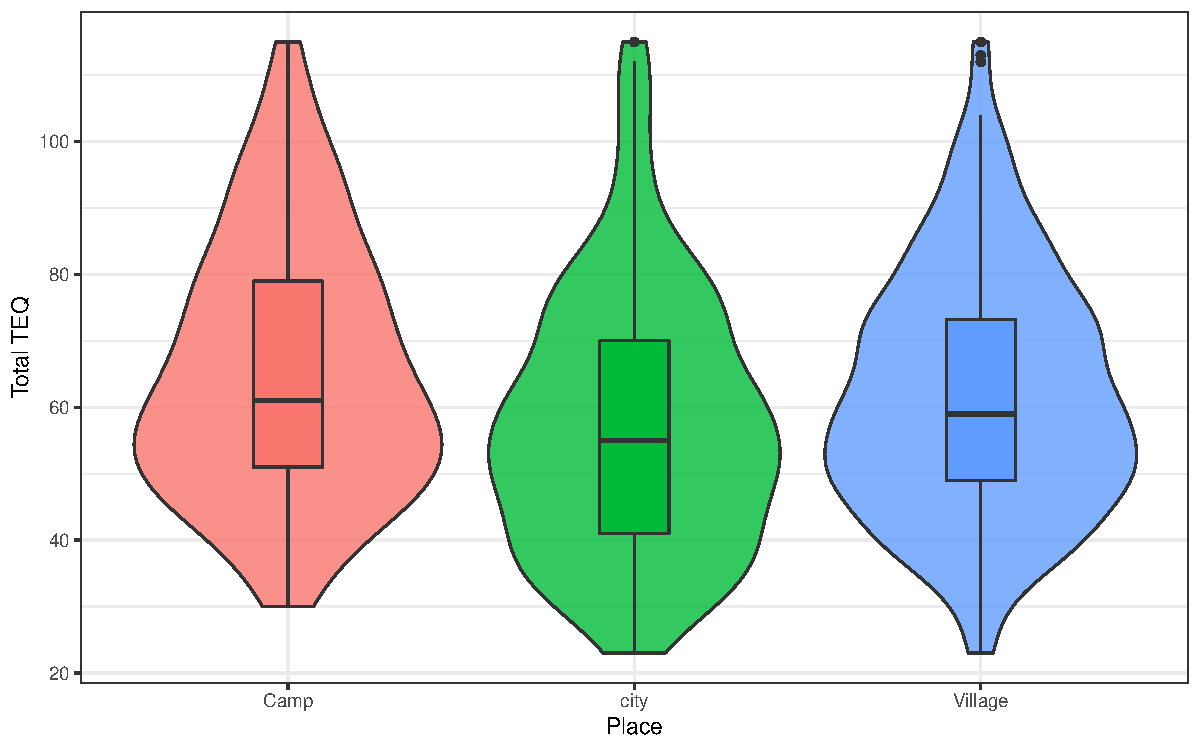
\includegraphics[width=1\linewidth]{04-s01-lab02a_files/figure-latex/graph2-1} 

}

\caption{TEQ Scores}\label{fig:graph2}
\end{figure}

From looking at the graph we just created, what location tends to have highest TEQ?

 Village Camp City

\hypertarget{recoding-factors}{%
\section{Recoding Factors}\label{recoding-factors}}

The original file has Camp, city, Village. It might be neater to have Camp, City, Village. We can easily recode the city level of the Place factor using the following code.

If you re-run the code for the graph now, this should be updated.

\begin{Shaded}
\begin{Highlighting}[]
\NormalTok{total_TEQ <-}\StringTok{ }\NormalTok{total_TEQ }\OperatorTok
\StringTok{    }\KeywordTok{mutate}\NormalTok{(}\DataTypeTok{Place =} \KeywordTok{recode}\NormalTok{(Place, }\DataTypeTok{city =} \StringTok{"City"}\NormalTok{))}
\end{Highlighting}
\end{Shaded}

\hypertarget{simple-network}{%
\section{Simple Network}\label{simple-network}}

When creating a network, it is important to think about how complex it will be. The higher the number of nodes being examined, then the higher the number of edges have to be estimated. Too many nodes results in networks that are unstable.

In this example, we will create a simple network from the single question items of the PAQ (Parental Authority Questionnaire).

First, we will select the PAQ items from data\_factors:

\begin{Shaded}
\begin{Highlighting}[]
\NormalTok{PAQ <-}\StringTok{ }\NormalTok{data_factors }\OperatorTok
\StringTok{  }\KeywordTok{select}\NormalTok{(PAQ1}\OperatorTok{:}\NormalTok{PAQ12)}
\end{Highlighting}
\end{Shaded}

Like all statistical techniques that use sample data to estimate parameters, the correlation and partial correlations values will be influenced by sampling variations and exact zeros will be rarely observed in the matrices. Consequently, correlation networks will nearly always be fully connected networks, possibly with small weights on many of the edges that reflect weak and potentially spurious partial correlations.

Spurious relationships will be problematic in terms of the network interpretation and will compromise the potential for network replication. In order to limit the number of such spurious relationships, a statistical regularisation technique, which takes into account the model complexity, is frequently used.

The LASSO regularisation yields a more parsimonious network (fewer connections between nodes), assumed to reflect only the most ``important'' empirical relationships in the data. The LASSO utilizes a tuning parameter λ (lambda) that controls the level of sparsity. The tuning parameter directly controls how much the likelihood is penalized for the sum of absolute parameter values. When the tuning parameter is low, only a few edges are removed, likely resulting in the retention of spurious edges. When the tuning parameter is high, many edges are removed, likely resulting in the removal of true edges in addition to the removal of spurious edges. EBICglasso sets a tuning parameter of 0.5 by default.

\begin{Shaded}
\begin{Highlighting}[]
\NormalTok{Network <-}\StringTok{ }\KeywordTok{estimateNetwork}\NormalTok{(PAQ, }\DataTypeTok{default =} \StringTok{"EBICglasso"}\NormalTok{, }\DataTypeTok{corMethod =} \StringTok{"cor_auto"}\NormalTok{)}
\end{Highlighting}
\end{Shaded}

The size and density of the edges between the nodes respresent the strength of connectedness. Positively related nodes are shown in { blue} and negatively related nodes are shown in {red}.

\begin{Shaded}
\begin{Highlighting}[]
\KeywordTok{plot}\NormalTok{(Network, }\DataTypeTok{layout=}\StringTok{"spring"}\NormalTok{, }\DataTypeTok{labels=}\KeywordTok{colnames}\NormalTok{(PAQ))}
\end{Highlighting}
\end{Shaded}

\begin{figure}

{\centering 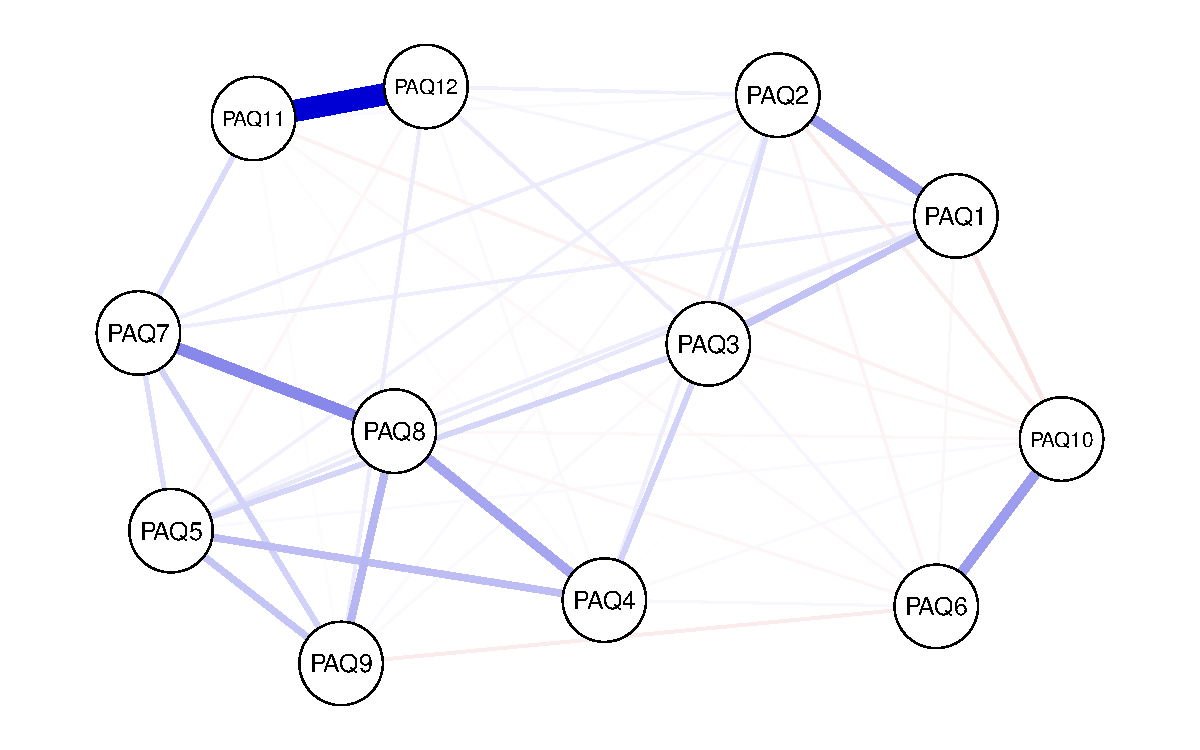
\includegraphics[width=1\linewidth]{04-s01-lab02a_files/figure-latex/Plotting-1} 

}

\caption{PAQ Network Graph}\label{fig:Plotting}
\end{figure}

\hypertarget{interpretation}{%
\section{Interpretation}\label{interpretation}}

The network shows the strength of relationships between the TPB variables. Some variables have quite strong connections (e.g.~PAQ12 and PAQ11), whereas others have weak relationship (e.g.~PAQ 7 and PAQ3). Visual inspection of the network suggests that some variables may be related. However, visual inspection of the graphical display of complex relationships requires careful interpretation, especially if there are a large number of nodes in the network.

A key concept in network analysis is the centrality of the symptom: if a behaviour or symptom (e.g.~fatigue) has many and/or strong associations to other nodes, they are more central within the network than a less connected symptom.There are different centrality metrics, and \emph{strength} most often used. Expected influence is related to strength but argued to be a \href{https://psych-networks.com/expected-influence-new-centrality-metric-robinaugh-et-al-2016/}{better metric} - adapted from open source materials by \href{https://derekdebeurs.github.io/esssb17/}{Derek DeBuers}

From looking at both strength and expected influence, it appears PAQ12 and PAQ8 have the strongest influence on the nodes in the network. How might we interpret this? Network analysis is purely statistical, the measurement and inclusion of nodes depend on your theory / research question.

\begin{Shaded}
\begin{Highlighting}[]
\KeywordTok{centralityPlot}\NormalTok{(Network, }\DataTypeTok{include =} \KeywordTok{c}\NormalTok{(}\StringTok{"Strength"}\NormalTok{,}\StringTok{"ExpectedInfluence"}\NormalTok{),}
               \DataTypeTok{orderBy =} \StringTok{"ExpectedInfluence"}\NormalTok{)}
\end{Highlighting}
\end{Shaded}

\begin{figure}

{\centering 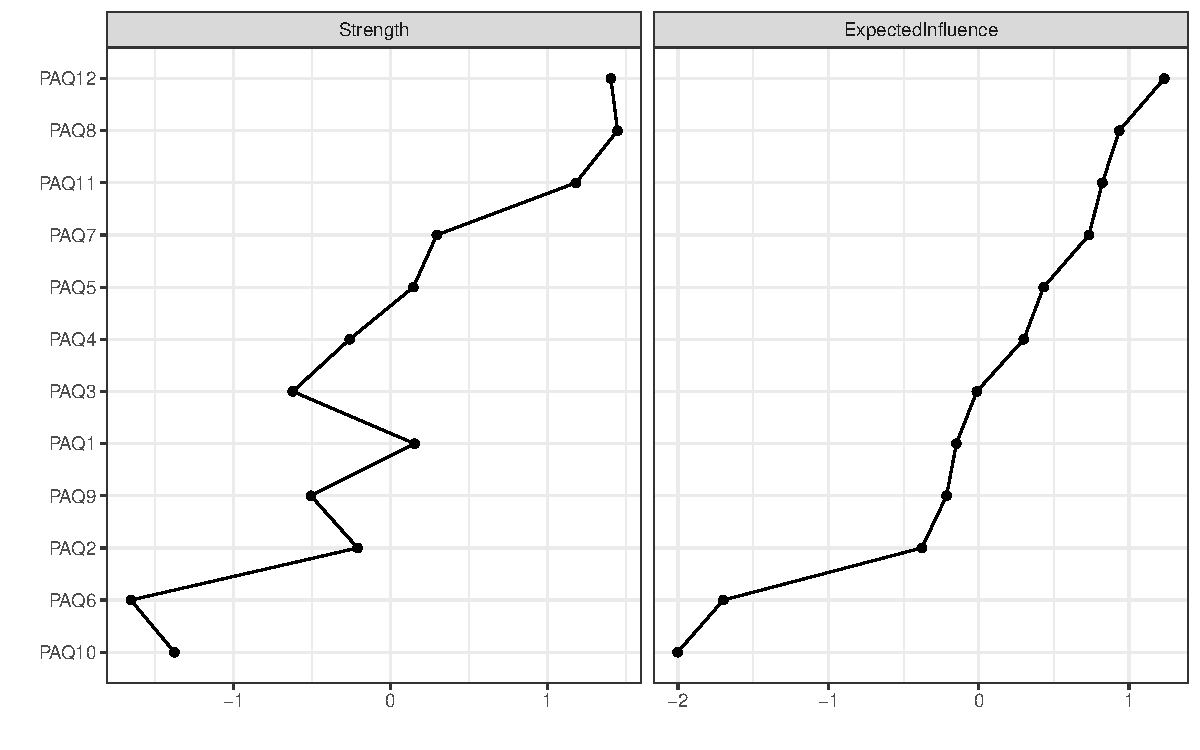
\includegraphics[width=1\linewidth]{04-s01-lab02a_files/figure-latex/Pcentrality-1} 

}

\caption{Centrality Plot}\label{fig:Pcentrality}
\end{figure}

\hypertarget{issues}{%
\section{Issues}\label{issues}}

This assumes normally disturbuted data which can be rare in psychology where Likert scales (such as that used to measure data here) are common.

``our data did not meet all assumptions of multivariate normality. This is not unusual in psychology, but as it is unclear at present how robust the employed methods are to such violations, results need to be interpreted with caution.'' \href{https://openaccess.leidenuniv.nl/bitstream/handle/1887/73951/Aalbers_et_al_2018_T.pdf?sequence=1}{(Aalbers, 2019)}

\hypertarget{appendix-appendices}{%
\appendix}


\hypertarget{rstudio-cloud}{%
\chapter{RStudio Cloud}\label{rstudio-cloud}}

Sometimes R might not work well on our own computers. However, there is an online version of R Studio (R Studio Cloud) which can be used in a pinch. Using R Studio Cloud is a little different to R Studio, so we have made a short guide to get you up and running.

\hypertarget{creating-an-account}{%
\section{Creating an Account}\label{creating-an-account}}

Head to \href{https://rstudio.cloud/}{RStudio Cloud} and click ``Sign Up'' at the top of the page

Enter details you wish to sign in with and select ``Sign up''

You'll receive an e-mail at the address you sign up with, make sure to click the link to activate your account fully.

\hypertarget{accessing-rstudio-cloud}{%
\section{Accessing RStudio Cloud}\label{accessing-rstudio-cloud}}

Head back to \href{https://rstudio.cloud/}{RStudio Cloud} and select ``log In'', where we previously chose ``Sign Up''

Once logged in, you'll be taken to the ``Your Workspace'' page, this is where all of your RStudio Cloud projects will be accessible from

Select ``New Project'' and then ``New Project'' again

You will see the message ``Deploying Project'' for a couple of minutes while it creates your Workspace

\hypertarget{getting-started-with-rstudio-cloud}{%
\section{Getting Started with RStudio Cloud}\label{getting-started-with-rstudio-cloud}}

Once loaded, you'll see a page that looks almost identical to the other screenshots in the learning material

\hypertarget{naming-the-workspace}{%
\subsection{Naming the Workspace}\label{naming-the-workspace}}

Let's give the project a better name!

Click on ``Untitled Project'' at the top of the page

This will allow you to rename to whatever you like, in this case we'll go for ``Network Training''

Press the return key on your keyboard, or click on a different area on the page to complete the task

\hypertarget{uploading-files}{%
\subsection{Uploading Files}\label{uploading-files}}

Since this is on the web, files on your computer won't be immediately accessible to RStudio Cloud, you will need to upload them yourself

Click the ``Upload'' button on the Files tab

An ``Upload Files'' element will load up where you can click ``Browse'' and select the file(s) you wish to make available to RStudio Cloud

Once you have selected a file and chosen ``OK'', you'll be taken back to the main application and you will now see the file you uploaded

You can now interact with this file as described in the rest of the learning material!

\hypertarget{references}{%
\chapter{References}\label{references}}

\href{http://sachaepskamp.com/files/Cookbook.html}{Network Analysis Cookbook - Also covers R introduction}

\href{https://psyteachr.github.io/}{We are grateful to PsyTeachR from the University of Glasgow} for allowing us to build upon their open source teaching materials.

\href{https://www.tandfonline.com/doi/full/10.1080/21642850.2018.1521283}{Network Analysis Tutorial}

\bibliography{book.bib,packages.bib}


\end{document}
